\documentclass[11pt,a4paper]{article}
\usepackage[utf8]{inputenc}
\usepackage[T1]{fontenc}
\usepackage{amsfonts}
\usepackage[french]{babel}
\frenchbsetup{StandardLists=true} % à inclure si on utilise \usepackage[francais]{babel}
\usepackage{enumitem}
\usepackage{amssymb}
\usepackage{amsmath}
\usepackage[left=2cm,right=2cm,top=2cm,bottom=2cm]{geometry}
\usepackage{multirow}
\usepackage[dvipsnames]{xcolor}

\usepackage{fouriernc}
\usepackage{graphicx}

\usepackage{setspace}
\singlespacing

\usepackage{pstricks}
\usepackage{xkeyval}
\usepackage{pst-labo}


\usepackage{multicol}
\usepackage{caption}
\usepackage{fancyhdr}
\pagestyle{fancy}
\renewcommand\headrulewidth{1pt}
\fancyhead[L]{Lycée Denis Diderot }
\fancyhead[R]{Classe de TMICRO}
\setcounter{page}{2}\fancyfoot[C]{page \thepage}
\fancyfoot[R]{Année 2025 2026}
\fancyfoot[L]{Alexis RUIZ}
\usepackage{multirow,tabularx,booktabs}
\newcommand{\cadreblanc}[1]{%
\medskip\framebox[\linewidth][c]{%
\rule{0mm}{#1mm}}\par
\medskip}
\setlength{\columnseprule}{.25mm}

\usepackage{awesomebox}
\setlength{\aweboxvskip}{0mm}
\usepackage{pifont}
\usepackage{chemmacros}
\chemsetup{modules=all}

\renewcommand{\arraystretch}{2}
\newcommand*\acocher{\quitvmode{\fboxsep0pt \fboxrule0.8pt \fbox{\vrule height1.8ex depth.1ex width0pt \vrule height0pt depth0pt width1.9ex }}}

\newcommand{\defproblem}{\awesomebox[black]{2pt}{\rotatebox{90}{\large{\textbf{Problématique}}}}{black}}
\newcommand{\defconclusion}{\awesomebox[black]{2pt}{\rotatebox{90}{\Large{\textbf{Conclusion}}}}{black}}

\frenchbsetup{StandardLists=true}
\begin{document}



\center \LARGE{TP1 - Déterminer la vitesse de propagation d'un son}
\\[0,3cm]

\normalsize

\hrule\
\\[0,2cm]

\flushleft \textbf{NOM :\\
Prénom:\\[0,2cm]
}
\hrule\
\\[0,2cm]

\defproblem{\begin{minipage}{14cm}
{
Camille et Sacha observent un orage à la fenêtre de leur appartement. Sacha constate que le bruit arrive en retard de 12 secondes par rapport à la lumière de l'éclair. Il dit que le son et la lumière ne se déplacent pas à la même vitesse.  \\
\begin{center}
\fbox{\textbf{Camille affirme que l'éclair s'est produit à 4 km, a-t-elle raison ? }}
\end{center}
}
\end{minipage}}

\vspace {1cm}

\ding{202} Calculer la vitesse de propagation du son dans l'air d'après les affirmations de Camille. \\
\cadreblanc{15}

\ding{203} Montage : réaliser le montage suivant\\
\begin{center}
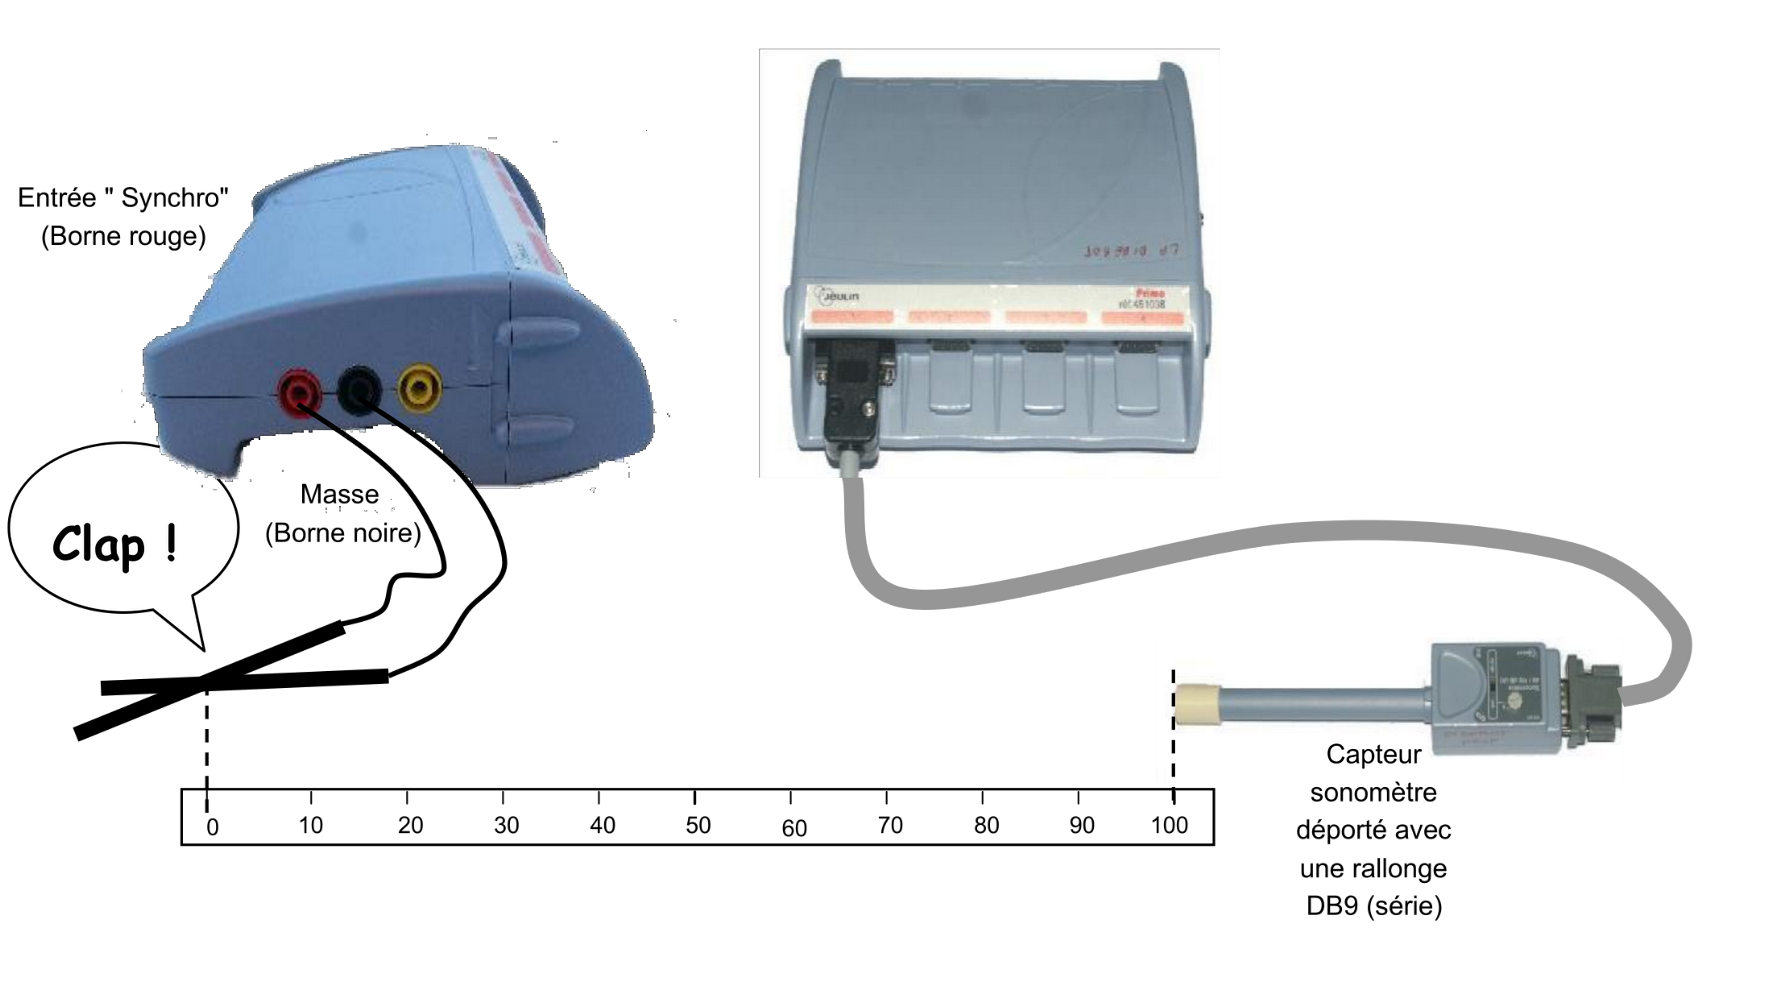
\includegraphics[scale=1]{images/montage exao TP1.png} 
\end{center}

\ding{204} Mesures\\
Lancer le module généraliste de l'Atelier scientifique Lycée Pro 
\begin{multicols}{2}
	\begin{center}
	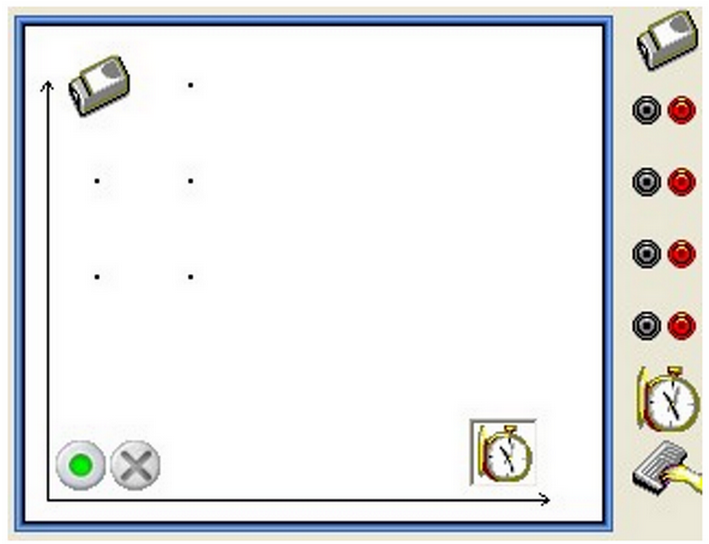
\includegraphics[scale=1]{images/MESURES 1 TP1.png} 
	\end{center}
	Faire glisser le capteur Sonomètre en entrée et le réveil en abscisse.
	\begin{center}
	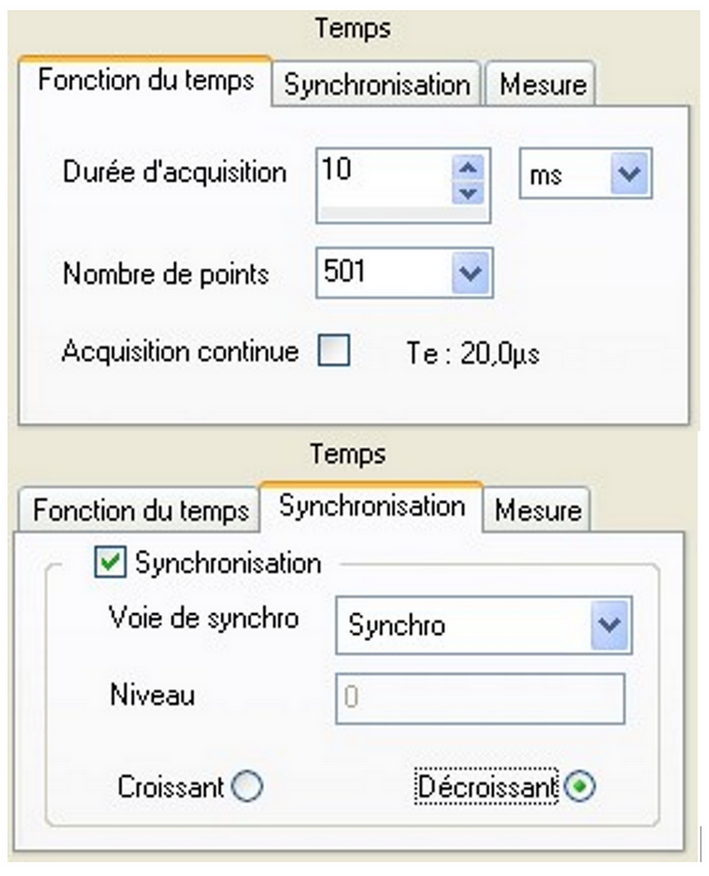
\includegraphics[scale=1]{images/MESURES 2 TP1.png} 
	\end{center}
	Cliquer sur le \textbf{réveil} en abscisse : 
	\begin{itemize}
		\item indiquer une durée de 10 ms.
		\item entrer 501 points
	\end{itemize}
	\vspace{1cm}
	Cliquer sur l'onglet \textbf{Synchronisation} : 
	\begin{itemize}
		\item cocher la case \textbf{Synchronisation}.
		\item sélectionner la voie \textbf{Entrée synchro}
		\item cocher le sens décroissant
	\end{itemize}
	Cliquer sur le feu vert puis sur Lancer, la console se met en attente de synchronisation.  


\end{multicols}
Taper fortement les 2 baguettes entre elles, ce qui provoque un déclenchement de la mesure.  
 
Enregistrer le fichier dans le répertoire personnel sous le nom "vitesse du son.lab"  
\vspace{5pt}

\ding{205} Exploitation : \\
 Sur le graphique, faire un clic droit et sélectionner l’outil Coordonnées \\ 
Placer le curseur sur le point de la courbe pour lequel le signal augmente brutalement, ce qui signifie que le signal sonore commence à être reçu par le capteur.  \\
Appuyer sur la touche Entrée : les coordonnées restent à l'écran. 
 
Dans la barre d'état s'affiche le décalage temporel t  à l'origine de la courbe initiale. \\
\textbf{Exemple : }
\begin{center}
\fbox{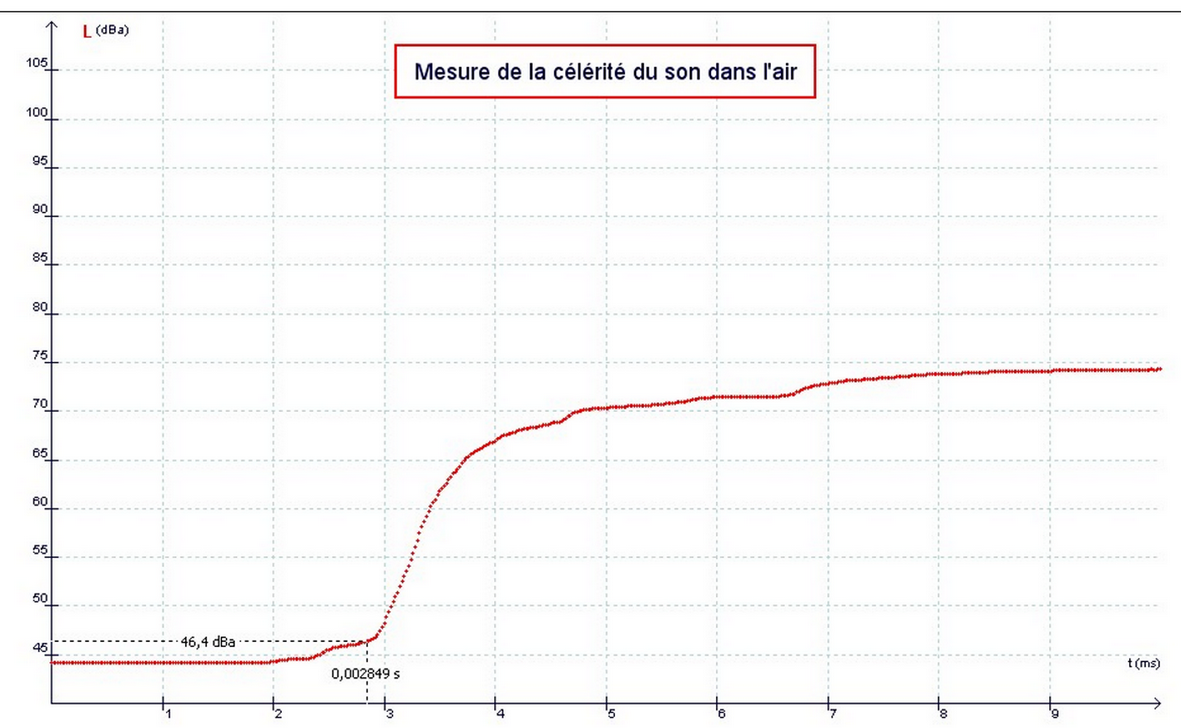
\includegraphics[scale=1]{images/graphique TP1.png} }
\end{center}
Calculer la vitesse du son dans l'air : 
\cadreblanc{20}

\ding{206} Conclusion : Proposer une méthode pour déterminer la distance où se situe un orage\\
\cadreblanc{30}
\end{document}